\section{Variação de temperatura}
Também podem ser determinados os esforços internos devidos a variações de temperatura que acontecem no elemento do sistema de equações~\ref{eq:caso1-Aii} ou \ref{eq:caso2-Aff}. Neste caso, impõem-se as condições $\mathbf{u}_I = \mathbf{u}_F = 0$, e substituem-se $\mathbf{u}_{I0}$ ou $\mathbf{u}_{F0}$ pelos vetores $\mathbf{u}_{It}$ ou $\mathbf{u}_{Ft}$, respectivamente, os quais são genericamente dados por:
\begin{equation}
	\label{eq:temp}
	u_{it} = \int_l \bar{M}_i d\beta_t + \int_l \bar{N}_i du_t, i=1,2,3\,\,\textrm{ou} \quad i=4,5,6.
\end{equation}

com
\begin{align}
	\label{eq:coeficientes1-temp}
	d\beta_t & = \dfrac{\alpha}{h(x_1)}(t_1-t_2)dx_1\,\,\,\textrm{(rotação flexional relativa)}                                  \\
	\label{eq:coeficientes2-temp}
	du_t     & = \alpha \left[ \dfrac{h_s(x_1)}{h(x_1)} (t_1-t_2) + t_2 \right]dx_1\,\,\,\textrm{(deslocamento axial relativo)},
\end{align}

onde $\alpha$ é o coeficiente de dilatação térmica, $t_1$ e $t_2$ são as variações de temperatura, e $h_s(x_1)$ e $h(x_1)$ são as funções de altura (ver figura~\ref{fig:el-acao-temperatura}). Escolhendo-se o sistema de equações~\ref{eq:caso1-Aii}, $\mathbf{u}_{It}$ é determinado, de modo que através das equações~\ref{eq:temp},~\ref{eq:coeficientes1-temp} e~\ref{eq:coeficientes2-temp}, obtém-se:

\begin{figure}[!htbp]
	\centering
	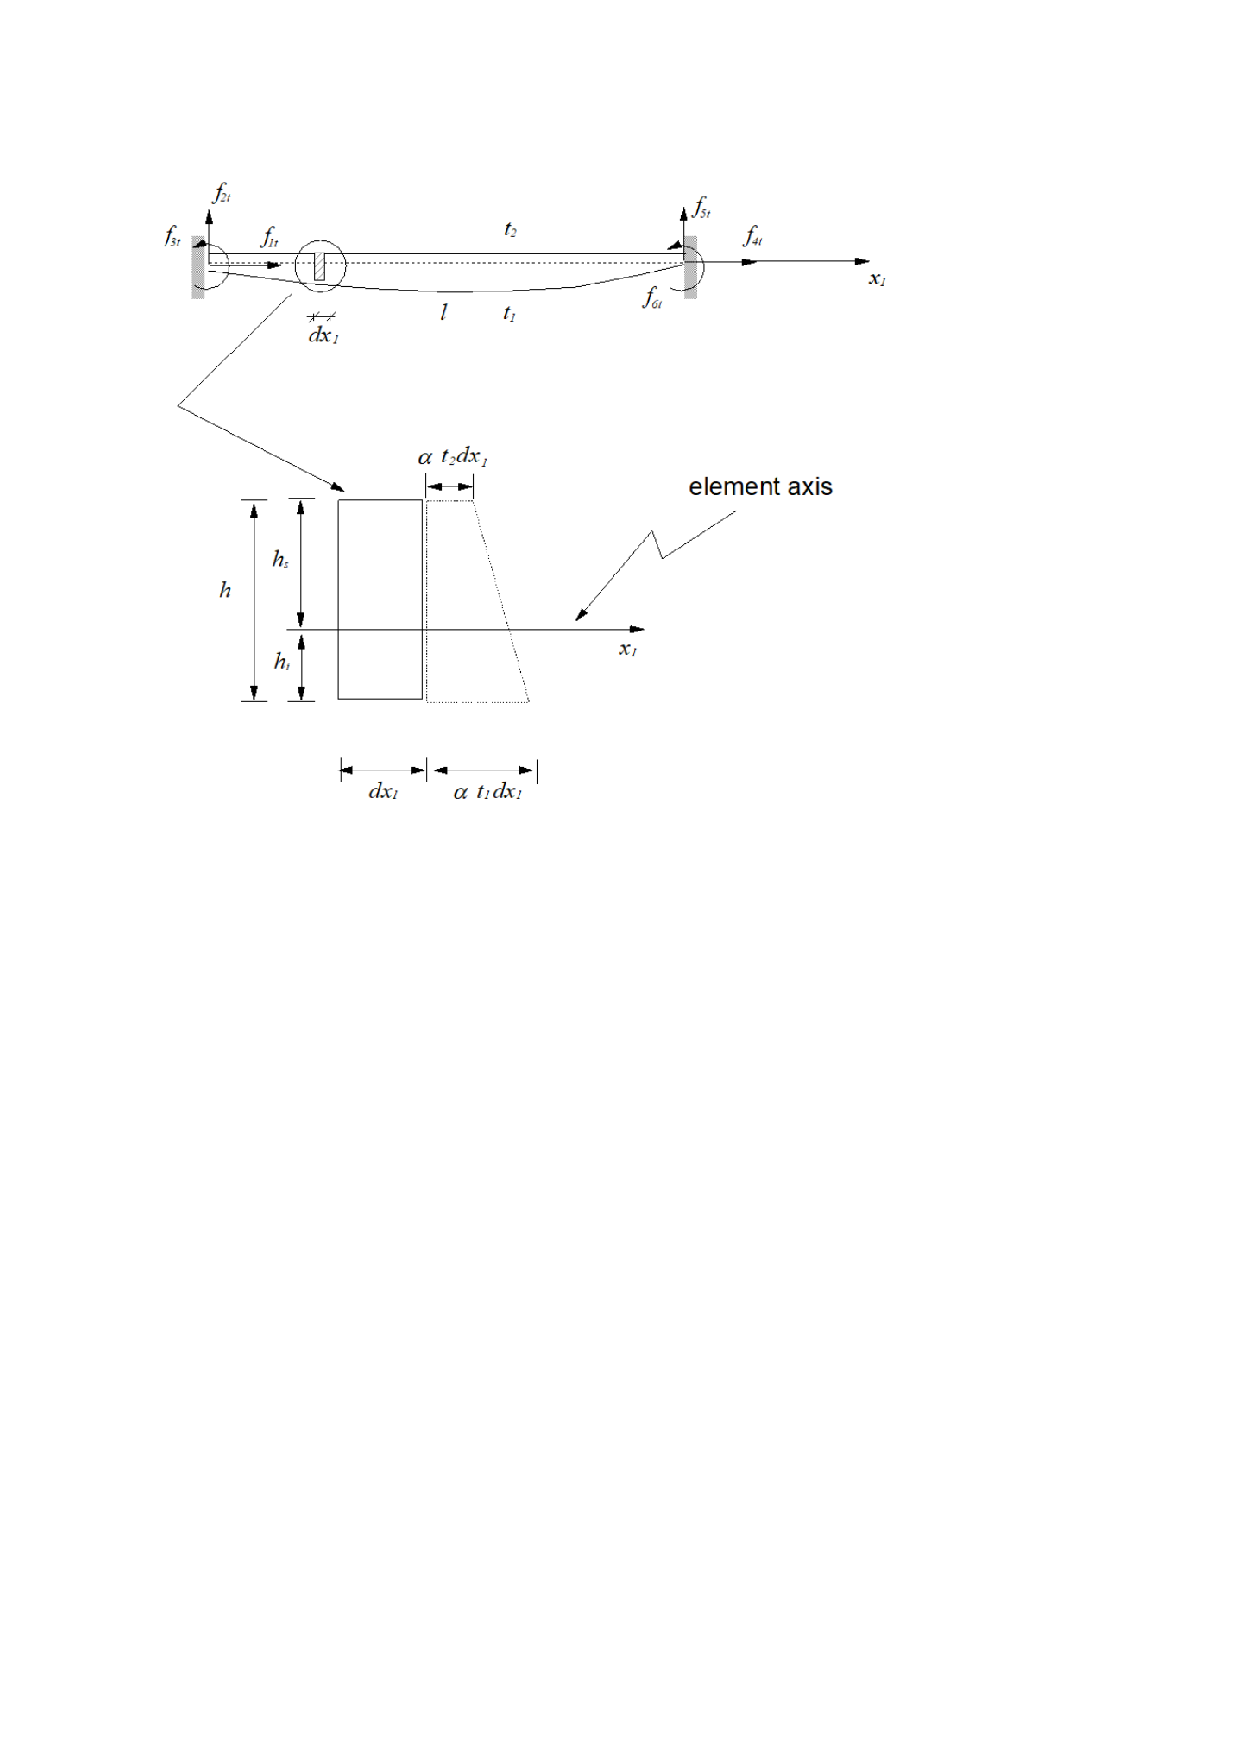
\includegraphics[trim = 20mm 160mm 60mm 25mm, clip, scale=1]{img/el-acao-temperatura.pdf}
	\caption{Elemento sob a ação de mudanças de temperatura}
	\label{fig:el-acao-temperatura}
\end{figure}

\begin{align}
	u_{1t} & = -\alpha \int_l \left[ \dfrac{h_s(x_1)}{h(x_1)} (t_1-t_2)+ t_2 \right]dx_1, \\
	u_{2t} & = \alpha \int_l \dfrac{x_1}{h(x_1)}(t_1-t_2)dx_1                             \\
	u_{3t} & = -\alpha \int \dfrac{(t_1-t_2)}{h(x_1)} dx_1
\end{align}

As ações de extremidade de membro $\mathbf{f}_{It}$ e $\mathbf{f}_{Ft}$ são portanto avaliadas resolvendo-se
\begin{equation}
	\begin{bmatrix}
		\mathbf{E}_{II} & \mathbf{E}_{IF} \\
		\mathbf{A}_{II} & \mathbf{0}
	\end{bmatrix}
	\begin{bmatrix}
		\mathbf{f}_{It} \\
		\mathbf{f}_{Ft}
	\end{bmatrix}
	=
	\begin{bmatrix}
		\mathbf{0} \\
		\mathbf{u}_{It}
	\end{bmatrix}
	.
\end{equation}